%!TEX root = ./main.tex

% content goes here 
    
    \section{Git}
	\begin{frame}
		\frametitle{Git}
		% \framesubtitle{}
		\begin{columns}[c]
    		\column{.5\textwidth} 
        		\begin{itemize}
					\item Collaborate
                    \item Version Control
                    \item Open Source
          		\end{itemize}
          	\column{.5\textwidth}
            	\centering
				
\includegraphics[width=.7\linewidth,]{res/git}

				\vspace{1cm} % blank lines around this are needed

				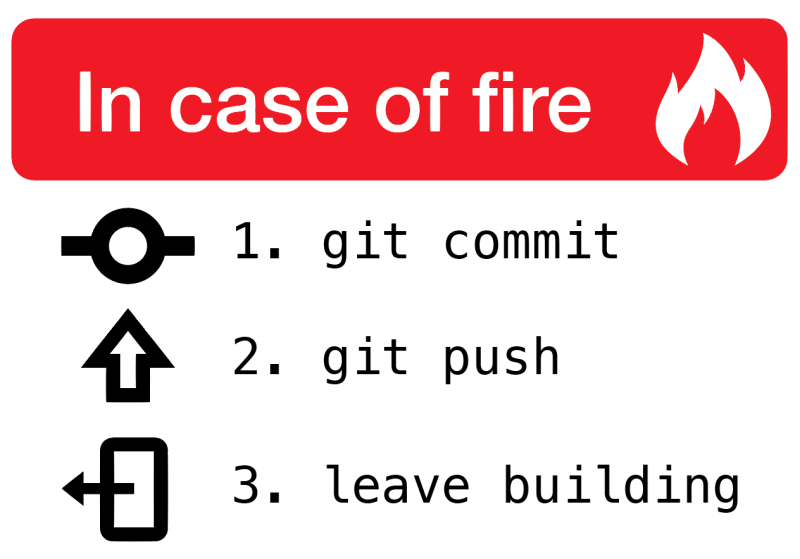
\includegraphics[width=.7\linewidth]{res/fire}
        \end{columns}
	\end{frame}
    
    \subsection{Workflow}
    \begin{frame}[allowframebreaks=10] % "=10" -> do not auto frame break
		\frametitle{Workflow}
		% \framesubtitle{}
        \begin{figure}
        	\centering
        	\includegraphics[width=0.8\linewidth]{"res/git_client-server"} \\
        \end{figure}
        \framebreak
        \begin{figure}
        	\centering
        	\includegraphics[width=0.8\linewidth]{"res/git_flow"}
        \end{figure}
	\end{frame}
    
    \subsection{Commands}
    \begin{frame} 
		\frametitle{Commands}
        \begin{tabularx}{\linewidth}{lX}
        	\textbf{git init}& Makes a new local repository \\ \vspace{0.05cm}
            \textbf{git clone {[}remote url{]}} & Clones into a remote repository \\ \vspace{0.05cm}
          	\textbf{git fetch}& Gets content from remote repo to local repo \\ \vspace{0.05cm}
            \textbf{git merge}& Merges local repo with working directory \\ \vspace{0.05cm}
            \textbf{git pull}& Shortcut for git fetch and git merge \\ \vspace{0.05cm}
            \textbf{git add {[}file{]}}& Puts file in the staging area \\ \vspace{0.05cm}
            \textbf{git commit} & Bundles files in staging area and sends them to local repo \\ \vspace{0.05cm}
            \textbf{git push}& Sends content from local repo to remote repo \\
        \end{tabularx}
        \begin{center}
        	\tcbox[colback=white, colframe=darkblue]{Remember: \textbf{man git {[}option{]}}}
        \end{center}
	\end{frame}
    
    \subsection{Demo}
    \begin{frame} 
		\frametitle{Demo}
        \begin{itemize}
        	\item Basic usage
            \item Merge conflicts
            \item Branches
            \item \href{https://try.github.io/}{Tutorial $\vcenter{\hbox{
\includegraphics[width=0.45cm]{res/link}}\vspace{0.1cm}}$}
        \end{itemize}
	\end{frame}
    
    \subsection{Branches}
    \begin{frame} 
		\frametitle{Branches}
        \begin{tabularx}{\linewidth}{lX}
        	\textbf{git branch} & Makes a new branch \\ \vspace{0.05cm}
            \textbf{git checkout} & Switches to branch \\ \vspace{0.05cm}
        \end{tabularx} \\
        \begin{figure}
        	\centering
        	\includegraphics[width=0.9\linewidth]{"res/git_branches2"}
        \end{figure}
	\end{frame}

	% end of content
